\documentclass[12pt]{article}
\usepackage{bookmark}
\usepackage{graphicx} 
\usepackage[german]{babel}
\usepackage{geometry}                % See geometry.pdf to learn the layout options. There are lots.
\geometry{letterpaper}                   % ... or a4paper or a5paper or ... 
\usepackage{graphicx}
\usepackage{amssymb}
\usepackage{amsthm}
\usepackage{epstopdf}
\usepackage[utf8]{inputenc}
\usepackage[usenames,dvipsnames]{color}
\usepackage[table]{xcolor}
\usepackage{hyperref}
\DeclareGraphicsRule{.tif}{png}{.png}{`convert #1 `dirname #1`/`basename #1 .tif`.png}

\theoremstyle{definition}
\newtheorem{example}{Example}

\newenvironment{explanation}{%
   \setlength{\parindent}{0pt}
   \itshape
   \color{blue}
}{}

\newcommand{\projectname}{Ship4You}
\newcommand{\productname}{Ship4You}
\newcommand{\projectleader}{Alexander Hrazdera/Paul Schöffl}
%\newcommand{\documentstatus}{In Arbeit}
\newcommand{\documentstatus}{Submitted}
%\newcommand{\documentstatus}{Released}
\newcommand{\version}{V. 1.0}

\begin{document}
\begin{titlepage}

\vspace{10em}

\begin{center}
{\Huge System Specification} \\[3em]
{\LARGE \productname} \\[3em]
\end{center}

\begin{flushleft} 
\begin{tabular}{|l|l|}
\hline
Projekt Name & \projectname \\ \hline
Projekt Leiter & \projectleader \\ \hline
Dokumenten Status & \documentstatus \\ \hline
Version & \version \\ \hline
\end{tabular}
\end{flushleft}

\end{titlepage}
\section*{Revisions}
\begin{tabular}{|l|l|l|}
\hline
\cellcolor[gray]{0.5}\textcolor{white}{Date} & \cellcolor[gray]{0.5}\textcolor{white}{Author} & \cellcolor[gray]{0.5}\textcolor{white}{Change} \\ \hline
November 03, 2019&A. Hrazdera/P. Schöffl&First version \\ \hline
\end{tabular}
\pagebreak
\tableofcontents
\pagebreak

\section{Initial Situation and Goal}
	Zu der Idee kamen wir über mehrere Personen, die uns mitteilten, dass sie so ein Programm schon öfters benötigt haben und uns fragten ob wir nicht so eines programmieren könnten. Also haben wir uns im Internet darüber informiert, ob es so eine Bewertungs-Website wirklich noch nicht in dieser Form gibt.
	Wir erkannten, dass es in diesem Bereich ein Deffizit gibt und dass solche Bewertungswebisten nur für AirBnB und der Gleichen zur Verfügung gestellt wurden.
	
	Aktuell kann beim Anmieten einer Yacht oder eines Segelbootes auf das Angebot verschiedener Vermieter (Vercharterer) nur so zugegriffen werden, dass der Mieter die einzelnen Websiten der Vercharterer besucht und sich das Angebot ansieht. Eine globale Suche von Booten in einer bestimmten Region ist derzeit nicht möglich.
	
	Weiters ist es noch nicht möglich, eine unabhängige Bewertung der Geschäfts\-trans\-aktion einer Vermietung (Zustand des Boots, Qualität der Betreuung, etc.) einzusehen. So ist man derzeit als Mieter noch von den Angaben des Vermieters abhängig und es ist schwierig bis unmöglich, sich ein eigenes und unabhängiges Bild zu machen. Dies gilt sowohl für die textuelle Beschreibung des Bootes als auch für die zur Verfügung gestellten Bilder.
	
	Auf der anderen Seite ist es für die Vercharterer auch sehr schwierig ihr Angebot an Booten zu kommunizieren. Jeder einzelne Vermieter muss sein Angebot auf seiner eigenen Website bewerben. Dies impliziert einen signifikanten Aufwand, der vor allem von Kleinvermietern nicht geleistet werden kann.
	
	Im Bereich der Ferienzimmervermietung oder auch Ferienwohnungsvermietung gibt es bereits ein Angebot an zentralen Plattformen (Airbnb, HomeAway, etc), welche einen niederschwellig zugänglichen Marktplatz für die Vermietung von Wohnungen und Zimmer ermöglicht.
	
	Vorteile:
	Mieter bekommt für sein Geld das bestmögliche Boot, weil er von anderen Usern die Bewertungen der Boote einsehen kann.
	
	Aufgrund der abgegebenen Bewertungen der User zu den Booten und dem Charterer, sinkt das Betrugsrisiko beträchtlich. Des weiteren helfen einem die hochgeladenen Bilder und Kommentare sich ein gutes Bild über das Boot zu machen.
	
	In weiterer Folge ist es sicherlich auch eine Erleichterung für den Vermieter. Dieser bekommt einen weiteren Platz sein Boot zu bewerben und erhält gleichzeitig ein konstruktives, hoffenlich gutes Feedback.
	
	Aufgund reger Nachfrage kann man dann auch Werbung auf unserer Website schalten. Potentielle Werbungspartner wären, Bootszubehör- bzw. Bootshändler und Städte mit Häfen.
	
	Risiko:
	Bewertungen können durch fehlerhafte Bilder bzw. Kommentare verfälscht werden. Aufgrund der Anmeldung versuchen wir den durch Bots verursachbaren Schaden möglichst klein zu halten.	

\subsection{Initial Situation}
	Der Einsatzbereich unserer Website liegt bei allen Menschen, die sich ein Boot mieten wollen, oder sich ein Boot gemietet haben und eine Bewertung dazu abgeben möchten.
	Auch können die Vermieter diese Website gut gebrauchen, um ihre Boote anzupreisen.
	Der Besitzer kann Aufgrund der Kommentare einsehen ob etwas mit dem zur Vermietung bereitgestellten Boot nicht passt. Somit ist unsere Website vielseitig einsetzbar.	

\subsubsection{Application Domain}
	Aktuell kann beim Anmieten einer Yacht oder eines Segelbootes auf das Angebot verschiedener Vermieter (Vercharterer) nur so zugegriffen werden, dass der Mieter die einzelnen Websiten der Vercharterer besucht und sich das Angebot ansieht. Eine globale Suche von Booten in einer bestimmten Region ist derzeit nicht möglich. 

	Weiteres ist es noch nicht möglich, eine unabhängige Bewertung der Geschäfts\-trans\-aktion einer Vermietung (Zustand des Boots, Qualität der Betreuung, etc.) einzusehen. So ist man derzeit als Mieter noch von den Angaben des Vermieters abhängig und es ist schwierig bis unmöglich, sich ein eigenes und unabhängiges Bild zu machen. Dies gilt sowohl für die textuelle Beschreibung des Bootes als auch für die zur Verfügung gestellten Bilder.
	
	Auf der anderen Seite ist es für die Vercharterer auch sehr schwierig ihr Angebot an Booten zu kommunizieren. Jeder einzelne Vermieter muss sein Angebot auf seiner eigenen Website bewerben. Dies impliziert einen signifikanten Aufwand, der vor allem von Kleinvermietern nicht geleistet werden kann. 
	
	Unser Programm sollte somit diesen fehlerhaften Marktanteil verschwinden lassen.

\subsubsection{Glossary}
	Der Vermieter (Vercharterer) kümmert sich um die Vermietung der Boote. Jedoch gehören diese Schiffe nicht ihm selber, sondern er bekommt diese von den Besitzern zur Verfügung gestellt.

	Der Besitzer selber stellt sein Boot dem Vermieter zur Verfügung, der sich um die Vermietung bzw. um das Bewerben der Boote kümmert. Dieser erhält vom Vermieter natürlich eine Provision dafür (Betrifft unsere Website jedoch nicht).
	Der Mieter der sich gerne ein Boot mieten möchte, kann auf unserer Website zu jenem Boot die Bewertungen einsehen. Des Weiteren kann er nach bestimmten Booten suchen.

\subsubsection{Model of the Application Domain}
	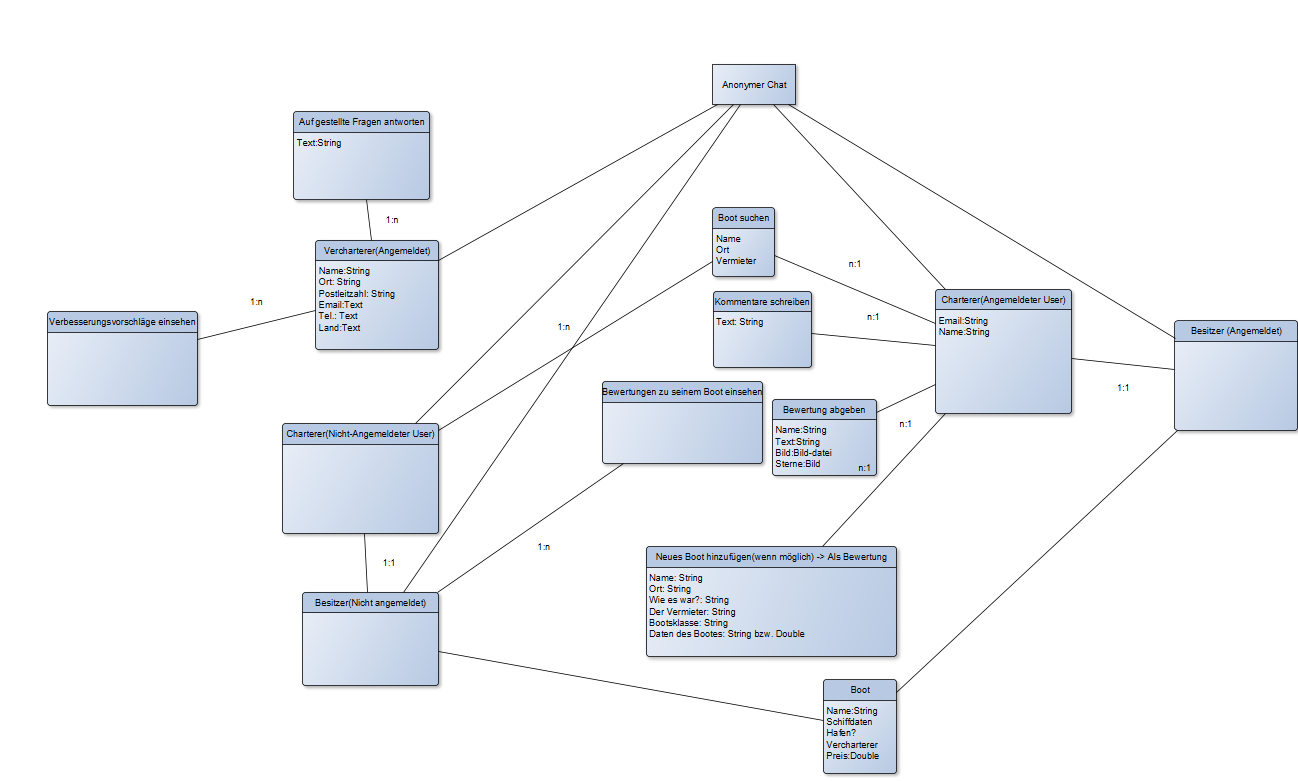
\includegraphics[height=0.50\textwidth]{SysUML.PNG}
	Die verschiedenen Userklassen(Gruppen) sind der Besitzer des Bootes (angemeldet bzw. nicht angemeldet), der Vercharterer (angemeldet) und der Charterer bzw. Ex Charterer oder auch normaler Website Besucher (angemeldet und nicht angemeldet).
	Der Besitzer des Bootes hat das Boot mit Namen, Schiffdaten, Hafen, Vercharterer und Preis. Dieser vermietet das Boot an den Vercharterer, der das Boot dann wiederrum zum Vermieten freigibt.  Der Besitzer kann sein Schiff und die Bewertungen dazu natürlich einsehen, um etwas zu kommentieren, muss er jedoch wie ein normaler Benutzer angemeldet sein.

	Der Vercharterer mit Namen, Ort, Postleitzahl, Email, Telefonnummer und Land, kann Verbesserungsvorschläge einsehen und auf diese eingehen. Des Weiteren kann er auf gestellte Fragen eingehen.

	Der Charterer(ohne Anmeldung) kann ein Boot nach den Suchkriterien (Name, Ort, Vermieter) suchen. Über einen anonymen Chat (siehe Willhaben.at) kann er mit dem Vercharterer bzw. dem Besitzer des Bootes in Kontakt treten. Er kann auch Bewertungen einsehen. Wenn der Charterer angemeldet ist, hat er die Möglichkeit, Kommentare zu schreiben und Bewertungen zu den Booten abzugeben. 

\subsection{Goal}
	Benutzer können sich anmelden, sind aber nicht dazu verpflichtet. Durch eine Anmeldung
	bekommen sie mehrere Features wie:
	\begin{itemize}
		\item Boote hochladen (Details der Boote, Bilder, …)
		\item Beschreibung abgeben
		\item Boote mieten
		\item Bewertungen schreiben, bearbeiten und löschen
		\item Anonymen Chat starten
	\end{itemize}
	Als unangemeldeter User kann man:
	\begin{itemize}
		\item nur Bewertungen lesen
		\item nach Booten suchen (nicht mieten)
	\end{itemize}
	Gesucht werden kann nach Ort, Vermieter, Schiffstyp und Schiffsname. Weiters ist es möglich Boote nach Preis, Größe, Bewertung und Namen zu filtern.
	Für Fragen steht ein anonymer Chat zur Verfügung, wo sich Vermieter und Mieter austauschen können. Bei Problemen steht ein freundlicher und hilfswilliger Support zur Verfügung. Wenn es weitere Infos gibt, können diese über Emails an das Team geschickt werden.
	Das Ziel dieses Projekts ist es möglichst viele Boote zur Verfügung zu stellen, damit sich Menschen, die gerne ein Boot mieten möchten, sich ein klares Bild von diesem Schiff machen können. Mithilfe der Zusammenarbeit ehrlicher Vermieter, können klar strukturierte Aussagen gemacht werden. Zum Beispiel ob ein Boot beschädigt ist, für eine bestimmte Anzahl an Personen geeignet ist oder das Boot dem angegeben Preis entspricht. Mit der Möglichkeit selbst Boote hochzuladen und eine Beschreibung bzw. Bewertung abzugeben soll anderen Personen geholfen werden, sich für das richtige Boot zu entscheiden. Es besteht weiterhin das Risiko, dass falsche Details zu Booten angegeben werden. Zur schnellen Übersicht werden die Boote mit der besten Bewertung angezeigt.
\pagebreak

\section{Functional Requirements}

\subsection{Overview}
	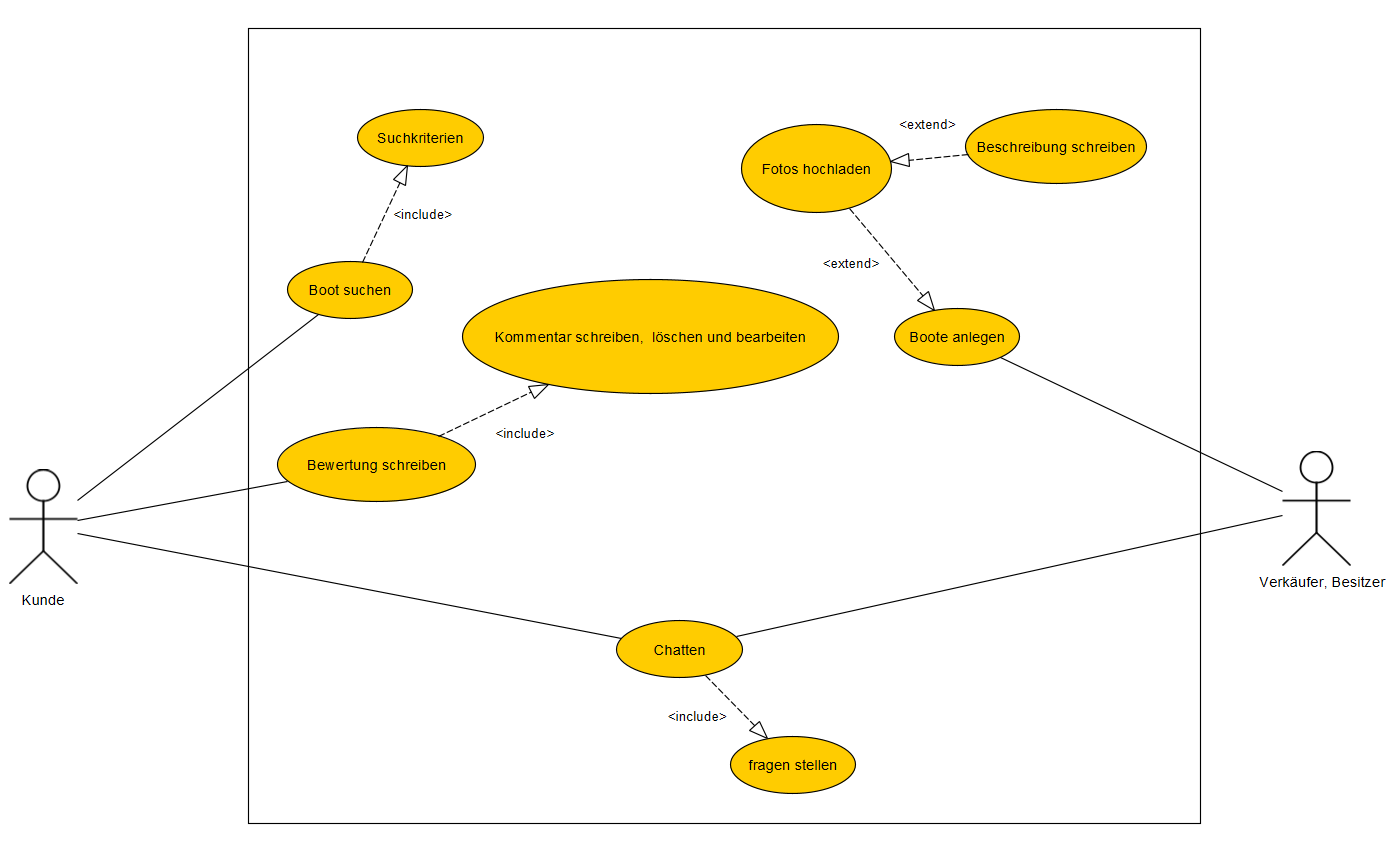
\includegraphics[height=0.50\textwidth]{UseCaseDiagram.PNG}
	\begin{itemize}
		\item UseCase 1: Der Kunde kann ein Boot suchen
		\item UseCase 2: Der Kunde kann eine Bewertung schreiben
		\item UseCase 3: Der Kunde bzw. der Verkäufer kann chatten bzw. mit dem Support schreiben
		\item UseCase 4: Der Verkäufer bzw. der Besitzer kann ein Boot anlegen 
	\end{itemize}

\subsection{Use Case 1: Boot suchen}
Der Kunde kann anhand von Suchkriterien ein Boot aus der Datenbank suchen.
\subsubsection{General Description}
	\begin{itemize}
		\item User gibt in einer Suchleiste den Namen des Bootes ein.
		\item User kann durch ankreuzen weitere Suchkriterien auswählen.
		\item Im Hintergrund wird eine Abfrage an die Datenbank geschickt.
		\item Der User bekommt die Boote, die zu seinen Suchkriterien passen.
	\end{itemize}

\begin{tabular}{|p{.2\linewidth}|p{.65\linewidth}|}
\hline 
ID: & 1 \\ \hline
Goal: & Der User sollte die Boote nach seinen Suchkriterien ausgelesen bekommen um Bewertungen, Kommentare und Bilder einsehen zu können. \\ \hline
Precondition: & Ist einer der Haupt-UseCases. Dieser wird benötigt um die Bootssuche zu verwenden. \\ \hline
Postcondition: & Die Bedinung das der User eine Liste von Booten bekommt ist dann als erfolgreich gekennzeichnet. \\ \hline
Involved Users: &Kunde: Der User sucht nach Suchkriterien ein auf ihn abgestimmtes Boot. \\ \hline
\end{tabular}

\subsubsection{UI to call the use case}
\begin{center}
\includegraphics[width=15cm,height=20cm,keepaspectratio]{Startseite2.png}\end{center}

\subsubsection{The Standard Use}
Wenn alles funktionier hat, werden dem User, der die Suche durchgeführt hat, die Boote angezeigt, die auf seine Suchkriterien abgestimmt sind.
\begin{itemize}
	\item UI: Suchfunktion
	\item Description: Man kann nach dem Ort, dem Vermieter, dem Schiffstyp und dem Schiffsnamen suchen. Wenn keine Daten gefunden werden bekommt der User eine Fehlermeldung.
	\item Activity, Sequence, or State Diagram to visualize the workflow
\end{itemize}
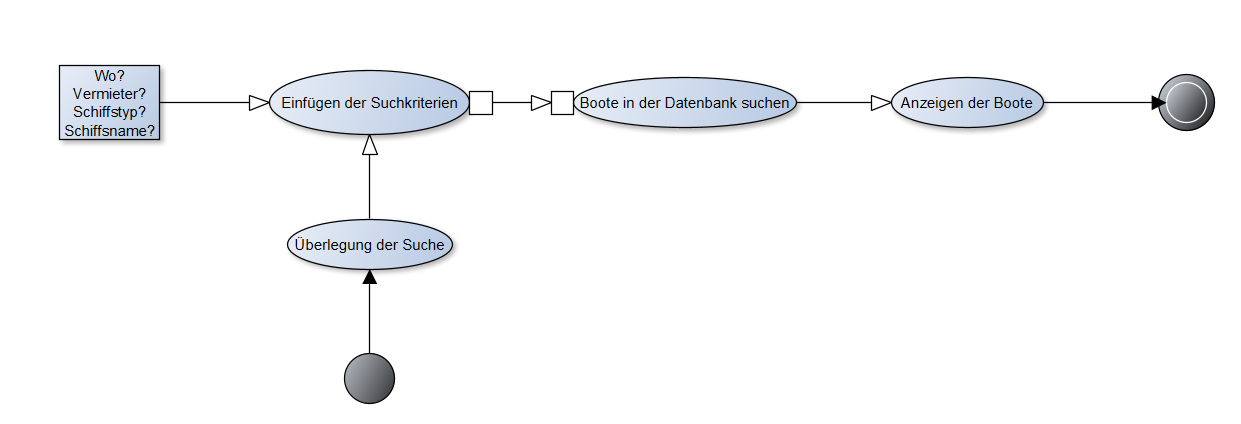
\includegraphics[height=0.40\textwidth]{Aktivitaetsdiagramm.PNG}

\subsubsection{The Non-Standard Use}
Es könnte sein, dass es keine Boote zu diesen Suchkriterien in der Datenbank gibt. Dieses wird dem User über eine Fehlermeldung mitgeteilt und er wird darum gebeten andere Suchkriterien zu verwenden.
\begin{itemize}
	\item UI: Fehlerseite es sind keine Boote vorhanden!
	\item Description: Es wird eine Fehlermeldung ausgegeben.
	\item Activity, Sequence, or State Diagram to visualize the workflow
\end{itemize}
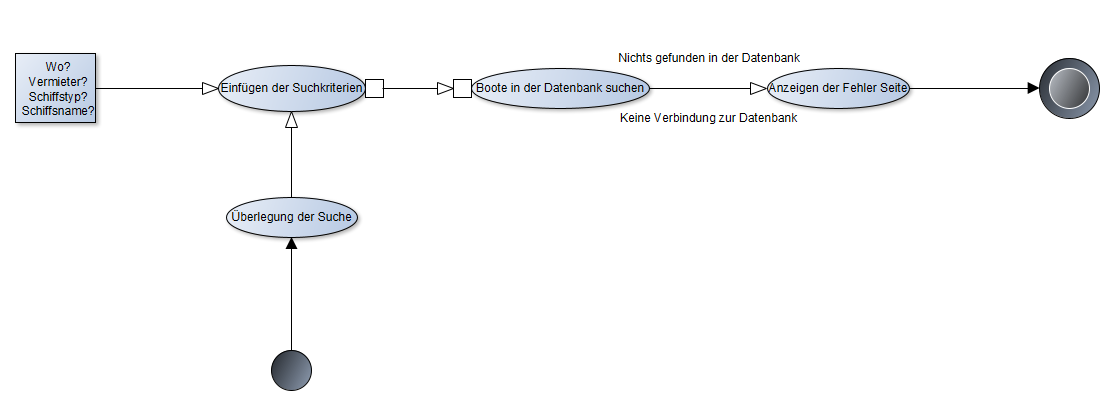
\includegraphics[height=0.40\textwidth]{Boote_Suchen_Fehler.PNG}
\begin{center}
\includegraphics[width=15cm,height=20cm,keepaspectratio]{Fehler_Suchen.PNG}\end{center}
\pagebreak

\subsection{Use Case 2: Bewertung schreiben}
Der Kunde kann zu jedem Boot einen Kommentar (eine kleine Berwertung) abgeben.
\subsubsection{General Description}
	\begin{itemize}
		\item Der User tippt auf einen Beitrag.
		\item Dort erscheind dann eine Kommentar bzw. Bewertungsfunktion.
		\item Dort kann er mit einer One-Click-Bewertung Sterne vergeben und per Hand einen kurzen Text schreiben.
	\end{itemize}

\begin{tabular}{|p{.2\linewidth}|p{.65\linewidth}|}
\hline 
ID: & 1 \\ \hline
Goal: & Der User sollte schnell, einfach und übersichtlich Kommentare und Bewertungen abgeben können. \\ \hline
Precondition: & Dieser UseCase wird benötigt um die Boote bewerten zu können (Ohne diese Funktion, würde die Website keinen Sinn machen). \\ \hline
Postcondition: & Der UseCase gilt dann als erfolgreich, wenn die Bewertung für andere User sichtbar ist. \\ \hline
Involved Users: &Kunde: Der User kann positive und negative Aspekte zu einem Boot abgeben. \\ \hline
\end{tabular}

\subsubsection{UI to call the use case}

\subsubsection{The Standard Use}
Wenn alles funktioniert hat, kann der User Kommentare und Bewertungen aufgeben, diese können dann auch von den anderen Usern eingesehen werden.
\begin{itemize}
	\item UI: Bewertung schreiben
	\item Description: Kunde kann eine Bewertung zu einem Boot abgeben. Bei einem Fehler erhält dieser eine Fehlermeldung.
	\item Activity, Sequence, or State Diagram to visualize the workflow
\end{itemize}
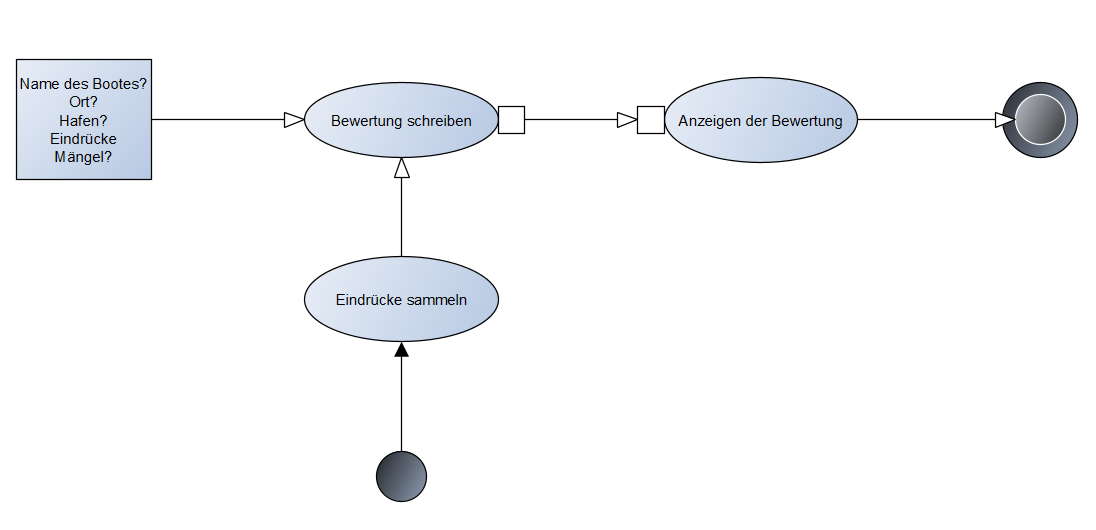
\includegraphics[height=0.40\textwidth]{Bewertung_schreiben.PNG}
\begin{center}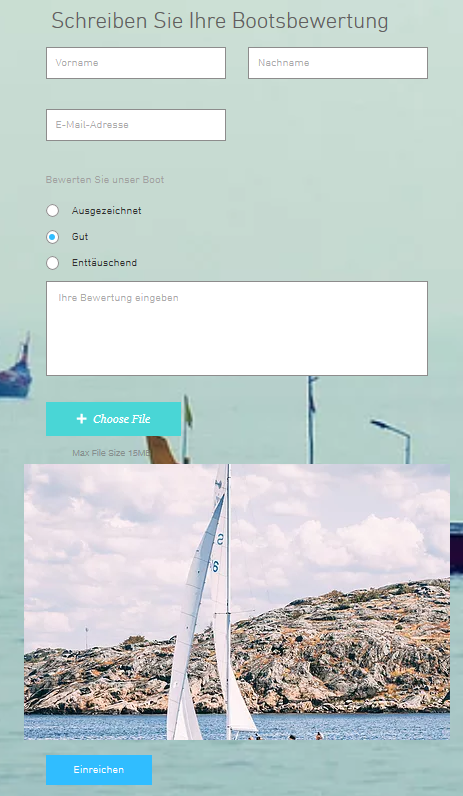
\includegraphics[width=10cm,height=15cm,keepaspectratio]{Bewertung_UI.PNG}\end{center}
\begin{center}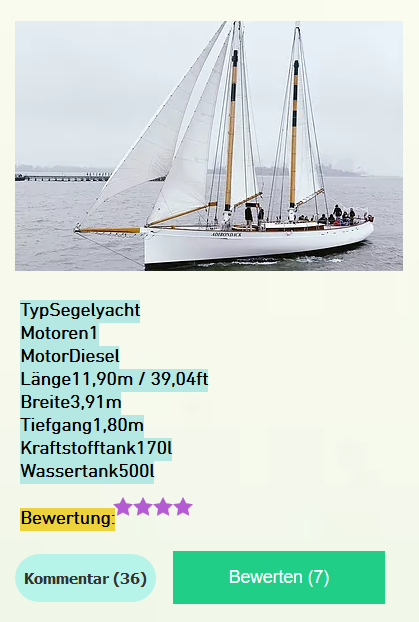
\includegraphics[width=10cm,height=15cm,keepaspectratio]{Bewerten.PNG}\end{center}

\subsubsection{The Non-Standard Use}
Es könnte sein, dass speichern der Bewertung in der Datenbank nicht funktioniert.
\begin{itemize}
	\item UI: Bewertung speichern Fehlerseite !
	\item Description: Es wird eine Fehlermeldung ausgegeben.
	\item Activity, Sequence, or State Diagram to visualize the workflow
\end{itemize}
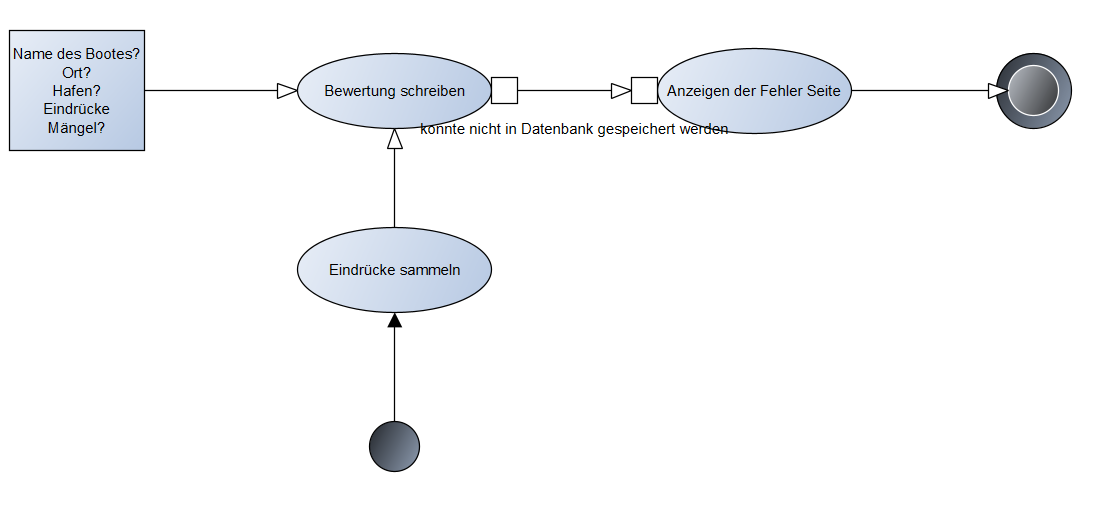
\includegraphics[height=0.40\textwidth]{Bewertung_schreiben_Fehler.PNG}
\begin{center}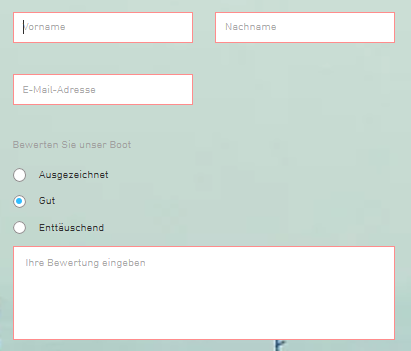
\includegraphics[width=10cm,height=15cm,keepaspectratio]{Bewertung_Pflichtfelder.PNG}\end{center}
\pagebreak

\subsection{Use Case 3: Chatten}
Der Kunde kann über einen anonymen Chat mit anderen Usern bzw. Vermietern in Kontakt treten.
\subsubsection{General Description}
	\begin{itemize}
		\item User klickt auf den Namen eines Users.
		\item Ein Chat-Fenster öffnet sich.
		\item Nun kann er sich mit dem anderen User austauschen.
	\end{itemize}

\begin{tabular}{|p{.2\linewidth}|p{.65\linewidth}|}
\hline 
ID: & 1 \\ \hline
Goal: & Dem User sollte es möglich sein, über einen Chat mit einem anderen in Kontakt zu treten. \\ \hline
Precondition: & Wird benötigt, um den Chat zu visualisieren. \\ \hline
Postcondition: & Wenn das Chat Fenster sich öffnet und das versenden bzw. empfangen der Nachricht funktioniert, gilt der Use-Case als abgeschlossen. \\ \hline
Involved Users: &Kunde: Die User können mit anderen Usern in Kontakt treten. \\ \hline
\end{tabular}

\subsubsection{UI to call the use case}

\subsubsection{The Standard Use}
Wenn alles funktioniert hat, können sich die User bei Fragen untereinander im Chat austauschen.
\begin{itemize}
	\item UI: Chat-UI
	\item Description: Der User kann per Mausklick mit einem anderen User in Kontakt treten. Es öffnet siche ein externes Fenster mit einem Chat. 
	\item Activity, Sequence, or State Diagram to visualize the workflow
\end{itemize}
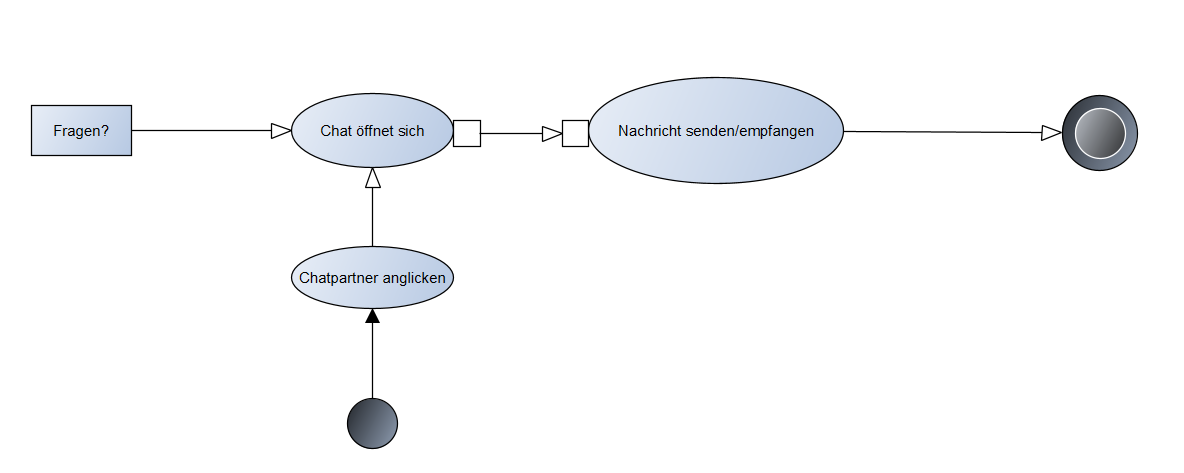
\includegraphics[height=0.40\textwidth]{Chatten.PNG}

\includegraphics[height=0.40\textwidth]{SupportChat.PNG}
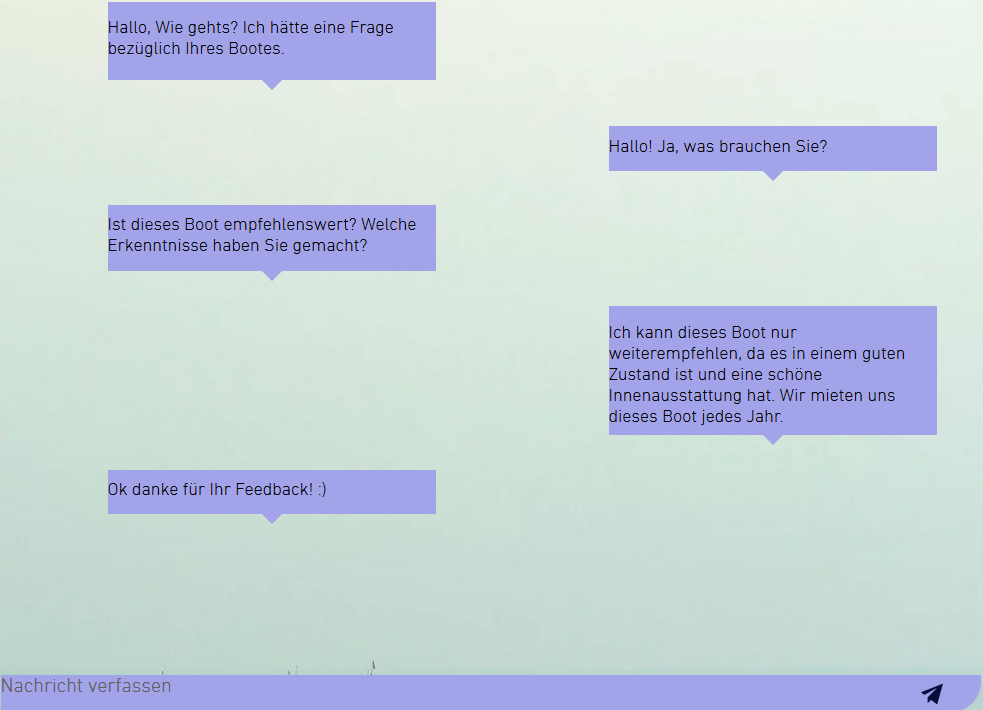
\includegraphics[height=0.40\textwidth]{Chat.PNG}

\subsubsection{The Non-Standard Use}
Es könnte sein, dass die Internetverbindung zu langsam für das senden der Nachricht ist. Somit wird dem User dieses als Fehlermeldung mitgeteilt.
\begin{itemize}
	\item UI
	\item Description: Erscheint, wenn ein Fehler auftritt.
	\item Activity, Sequence, or State Diagram to visualize the workflow
\end{itemize}
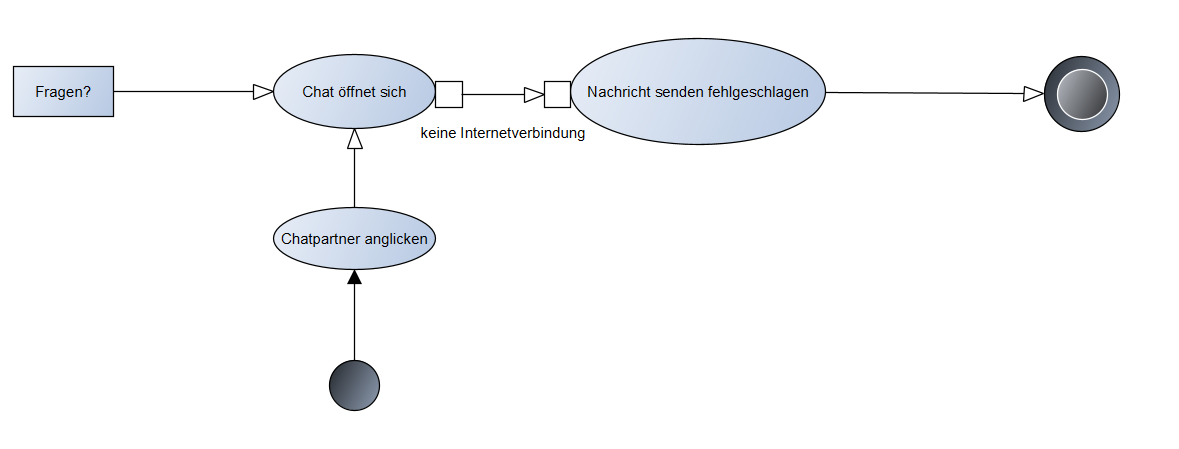
\includegraphics[height=0.40\textwidth]{Chatten_Fehler.PNG}
\begin{center}
\includegraphics[width=15cm,height=20cm,keepaspectratio]{Fehler2.PNG}\end{center}
\pagebreak


\subsection{Use Case 4: Boote anlegen}
Der Kunde kann neue Boote anlegen, zu diesem können dann die Bewertungen geschrieben werden.
\subsubsection{General Description}
	\begin{itemize}
		\item User klickt auf einen Button mit "neues Boot anlegen".
		\item Ein neues Fenster mit einer vorgegebenen Maske öffnet sich.
		\item Hier kann der User Bilder und Daten des Bootes eintragen und eine Bewertung, wenn er möchte, abgeben.
	\end{itemize}

\begin{tabular}{|p{.2\linewidth}|p{.65\linewidth}|}
\hline 
ID: & 4 \\ \hline
Goal: & Dem User sollte es möglich sein, ein neues Boot anzulegen. \\ \hline
Precondition: & Wird benötigt, um die Boote später bewerten zu können. \\ \hline
Postcondition: & Der Use-Case gilt als abgeschlossen, sobald ein neues Boot in der Datenbank eingelesen wurde.\\ \hline
Involved Users: &Kunde: Kann ein neues Boot anlegen. \\ \hline
\end{tabular}

\subsubsection{UI to call the use case}

\subsubsection{The Standard Use}
Wenn alles funktioniert hat, erscheint das Boot nach der Suche.
\begin{itemize}
	\item UI: Boot anlegen.
	\item Description: Der User kann, wenn er auf den Button "neues Boot anlegen" drückt, ein Boot hinzufügen. Es öffnet sich ein neues Fenster mit einer schon vorgegebenen Demo-Maske. 
	Nachdem speichern wird das Boot und dessen Daten in die Datenbank gespeichert. Bei einem Fehler wird eine Fehlermeldung ausgegeben.
	\item Activity, Sequence, or State Diagram to visualize the workflow
\end{itemize}
\begin{center}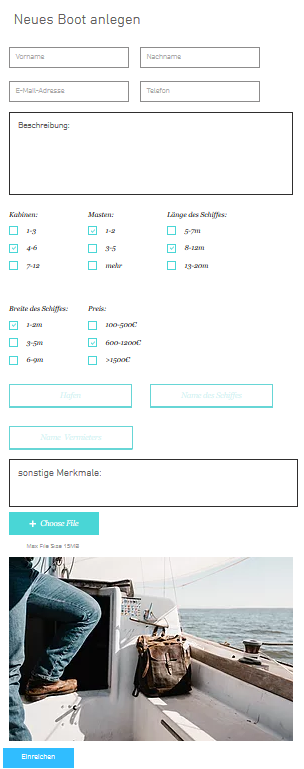
\includegraphics[width=10cm,height=15cm,keepaspectratio]{Boot_anlegen_UI.PNG}\end{center}

\subsubsection{The Non-Standard Use}
Es könnte sein, dass das Boot nicht in die Datenbank gespeichert wird.
\begin{itemize}
	\item UI: Fehlerseite - Boot anlegen!
	\item Description: Fehlermeldung, wenn das Speichern des Bootes in die Datenbank nicht funktioniert.
	\item Activity, Sequence, or State Diagram to visualize the workflow
\end{itemize}
\begin{center}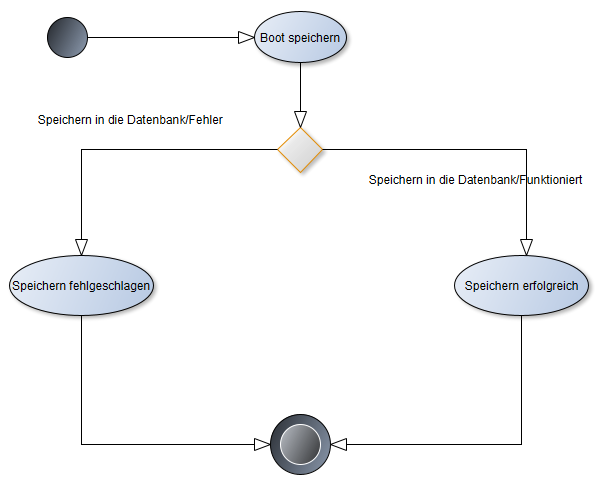
\includegraphics[width=15cm,height=20cm,keepaspectratio]{Boot_anlegen_Fehler.PNG}\end{center}
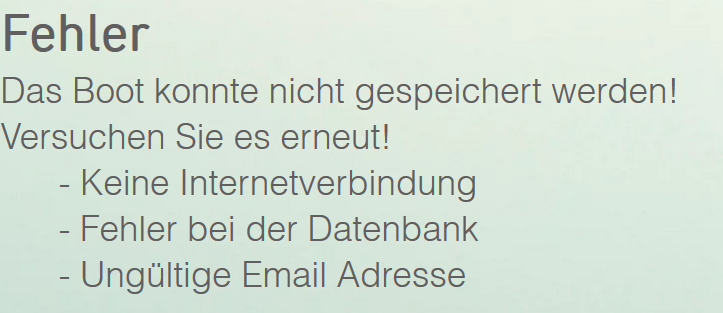
\includegraphics[height=0.40\textwidth]{Boot_anlegen-Fehler.PNG}
\pagebreak

\section{Non-Functional Requirements}

\subsection{NFR 1: Suche}
\begin{tabular}{|p{.2\linewidth}|p{.65\linewidth}|}
\hline 
ID: & 1 \\ \hline
Name: & Suche \\ \hline
Type	: & EFFIC \\ \hline
Descritpion: &  Die Suche sollte innerhalb von 1,5 Sekunden die Boote aus der Datenbank ausgelesen und diese auch dem User angezeigt haben.\\ \hline
\end{tabular}

\subsection{NFR 2: Bewertung schreiben}
\begin{tabular}{|p{.2\linewidth}|p{.65\linewidth}|}
\hline 
ID: & 2 \\ \hline
Name: & Bewertung schreiben \\ \hline
Type	: & USE \\ \hline
Descritpion: &  Das schreiben einer Bewertung sollte mit einem Klick möglich sein. (Eine Sterne-Bewertung für einen Beitrag abgeben). Jedoch kann man auch ein neues Boot Bewerten (hierzu sind Bilder, und ein kleiner Artikel nötig. (ca. 100 Textzeichen))\\ \hline
\end{tabular}

\subsection{NFR 3: Chatten}
\begin{tabular}{|p{.2\linewidth}|p{.65\linewidth}|}
\hline 
ID: & 3 \\ \hline
Name: & Chatten \\ \hline
Type	: & SEC und USE \\ \hline
Descritpion: &  Das chatten sollte Anonym ablaufen. Der User muss keine Daten bekannt geben (keine Telefonnummer, kein Name). \\Die verwendung des Chattes sollte per On-Cklick funktionieren. \\ \hline
\end{tabular}

\subsection{NFR 4: Boot anlegen}
\begin{tabular}{|p{.2\linewidth}|p{.65\linewidth}|}
\hline 
ID: & 4 \\ \hline
Name: & Boot anlegen \\ \hline
Type	: & USE \\ \hline
Descritpion: &  Beim Anlegen eines neuen Bootes sollte schon eine Vorgegebene Maske (Folie) zur Verfügung stehen. In diese man nur noch die Daten des Schiffes und seine Bewertung bzw. einen kleinen Text (100 Textzeichen) hinzufügen muss.\\ \hline
\end{tabular}
\pagebreak

\section{Quantity Structure}
Da die ganzen Beiträge (Die Boote mit (Name, Bewertungen, Kommentare, Texte, Bilder)) den größten Umfang der Website beanspruchen, werden wir hierfür eine Datenbank benutzen. In dieser wir jede Bootbewertung übersichtlich gliedern bzw. einteilen können.

\pagebreak
\section{System Architecture and Interfaces}
Unser System ist für die Kunden vorerst nur über eine Website verfügbar. Später wird vielleicht auch eine App zur besseren Nutzung auf den Mobiltelephonen zur verfügung stehen. Unsere Website greift auf eine Datenbank wo die Boote gespeichert sind zu. Des Weiteren werden wir einen automatischen Email-Sender implementieren, um Passwörter leichter zurücksetzen zu können.

\pagebreak
\section{Acceptance Criteria}
Suche:
\begin{itemize}
	\item Die Suche muss schnell (1,5s) und zuverlässig funktionieren
\end{itemize}
Boot anlegen:
\begin{itemize}
	\item Das Boot anlegen muss einfach und übersichtlich funktionieren. Die vorgabe Folie sollte schön gestaltet sein.
\end{itemize}
Chat
\begin{itemize}
	\item Der Chat sollte schnell (1,5s) und ohne verzögerung funktionieren.
\end{itemize}
\cite{endLine}
\bibliography{my_bib}{}
\bibliographystyle{plain}
\end{document}  